\documentclass[dvisvgm, tikz, border=4pt]{standalone}
\begin{document}
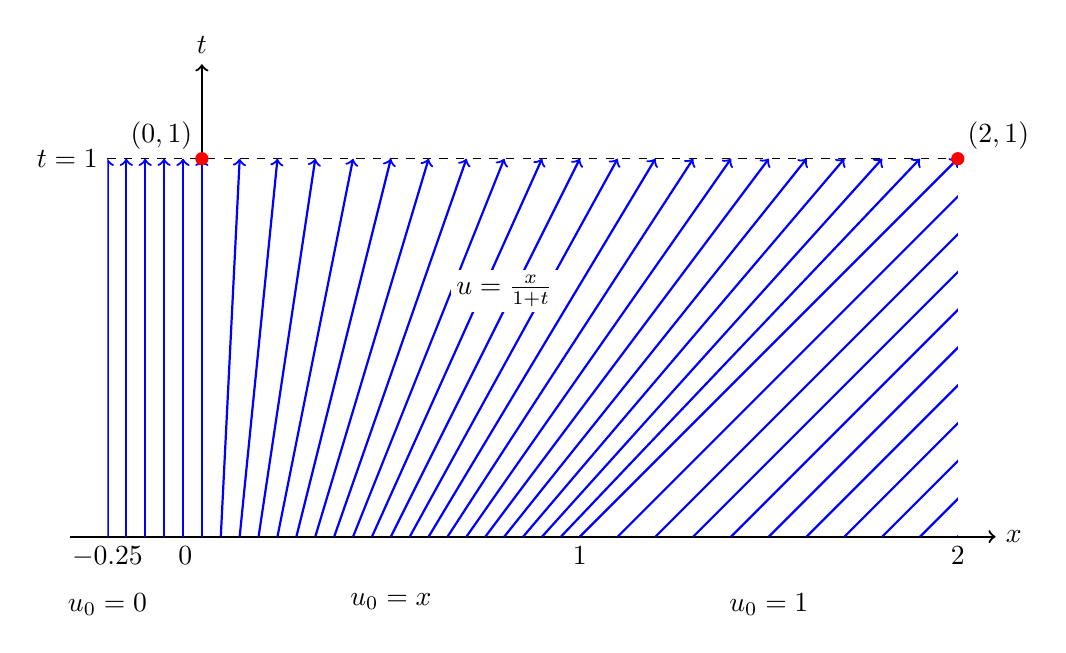
\begin{tikzpicture}[scale=1.2]
  % Display coordinates: X=4x, T=4t.
  \draw[->,thick] (-1.4,0) -- (8.4,0) node[right] {$x$};
  \draw[->,thick] (0,0) -- (0,5) node[above] {$t$};

  \draw[dashed] (-1,4) -- (8,4);
  \node[left] at (-1,4) {$t=1$};

  \begin{scope}
    \clip (-1,0) rectangle (8,4);

    % Left parallel characteristics (u_0 = 0).
    \foreach \k in {0,...,5}{
      \pgfmathsetmacro{\a}{-0.2*\k}
      \draw[blue,thick,->] (\a,0) -- (\a,4);
    }

    % Expanding characteristics: x = a(1+t).
    \foreach \k in {1,...,19}{
      \pgfmathsetmacro{\a}{0.2*\k}
      \draw[blue,thick,->] (\a,0) -- ({2*\a},4);
    }

    % Right parallel characteristics (u_0 = 1).
    \foreach \k in {0,...,10}{
      \pgfmathsetmacro{\a}{4+0.4*\k}
      \draw[blue,thick,->] (\a,0) -- ({\a+4},4);
    }
  \end{scope}

  % Edges of the expansion wave at t=1.
  \fill[red] (0,4) circle (2pt);
  \fill[red] (8,4) circle (2pt);
  \node[above left]  at (0,4) {$(0,1)$};
  \node[above right] at (8,4) {$(2,1)$};

  % Solution inside the wave.
  \node[fill=white,inner sep=2pt] at (3.2,2.6) {$u=\frac{x}{1+t}$};

  % Physical coordinates.
  \node[below] at (-1,0) {$-0.25$};
  \node[below left] at (0,0) {$0$};
  \node[below] at (4,0) {$1$};
  \node[below] at (8,0) {$2$};

  % Initial data.
  \node[below] at (-1,-0.5) {$u_0=0$};
  \node[below] at (2,-0.5) {$u_0=x$};
  \node[below] at (6,-0.5) {$u_0=1$};
\end{tikzpicture}
\end{document}
